\chapter{What is Perceptron?}
In machine learning, the perceptron is an algorithm for supervised classification of an input into one of several possible non-binary outputs. It is a type of linear classifier, i.e. a classification algorithm that makes its predictions based on a linear predictor function combining a set of weights with the feature vector. The algorithm allows for online learning, in that it processes elements in the training set one at a time.

The perceptron algorithm dates back to the late 1950s; its first implementation, in custom hardware, was one of the first artificial neural networks to be produced.

\section{A Bit of History}
The perceptron algorithm was invented in 1957 at the Cornell Aeronautical Laboratory by Frank Rosenblatt, funded by the United States Office of Naval Research. \hfill \\

More on the web!

\section{Definition}
In the modern sense, the perceptron is an algorithm for learning a \textbf{binary classifier}: a function that maps its input x (a real-valued vector) to an output value f(x) (a single binary value):

\[ f(x) = \left\{ 
               \begin{array}{l l}
                1  : & \quad w.x+b > 0 \\
                0  : & \quad otherwise
               \end{array} 
       \right.
\]

where...
\begin{itemize}
%\itemsep0em 
\item $\mathbf{w}$ is a vector of real-valued weights, 
\item $\mathbf{w \cdot x}$ is the dot product (which here computes a weighted sum), and $\mathbf{b}$ is the 'bias', 
\item a constant term that does not depend on any input value.
\end{itemize}

If $b$ is negative, then the weighted combination of inputs must produce a positive value greater than $|b|$ in order to push the classifier neuron over the 0 threshold. Spatially, the bias alters the position (though not the orientation) of the decision boundary. The perceptron learning algorithm does not terminate if the learning set is not linearly separable. If the vectors are not linearly separable learning will never reach a point where all vectors are classified properly. The most famous example of the perceptron's inability to solve problems with linearly nonseparable vectors is the Boolean exclusive-or problem.

In the context of neural networks, a perceptron is an \textbf{artificial neuron} using the \textbf{Heaviside step function} as the activation function. The perceptron algorithm is also termed the \textbf{single-layer perceptron}, to distinguish it from a multilayer perceptron, which is a misnomer for a more complicated neural network. As a linear classifier, the single-layer perceptron is the \textbf{simplest feedforward neural network}.

\section{Learning Algorithm}
Below is an example of a learning algorithm for a (single-layer) perceptron. For multilayer perceptrons, where a hidden layer exists, more sophisticated algorithms such as \textbf{backpropagation} must be used. Alternatively, methods such as the \textbf{delta rule} can be used if the function is \textbf{non-linear} and \textbf{differentiable}, although the one below will work as well.

When multiple perceptrons are combined in an artificial neural network, each output neuron operates independently of all the others; thus, learning each output can be considered in isolation.

\subsubsection{Definition}
We first define some variables:
\begin{itemize}
\item $y = f(\vec{\mathbf{z}})$ \, denotes the output from the perceptron for an input vector $\vec{\mathbf{z}}$.
\item $\mathbf{b}$ \, is the bias term, which in the example below we take to be 0.
\item $D = \{\vec{\mathbf{X}}_1,d_1)$,$\dots$,$(\vec{\mathbf{X}}_s,d_s)\}$ \, is the training set of s samples, where:
\begin{itemize}
\item $\vec{\mathbf{X}}_j$ is the n-dimensional input vector.
\item $\mathbf{d_j}$ \, is the desired output value of the perceptron for that input. \hfill \\
\end{itemize}

We show the values of the features as follows:
\item $x_{j,i}$ \, is the value of the ith feature of the jth training input vector.
\item $x_{j,0} = 1$ \,. 

\hfill \\ To represent the weights:
\item $w_i$ \, is the $i$th value in the weight vector, to be multiplied by the value of the $i$th input feature.
\item Because $x_{j,0}$ = 1 \,, the $w_0$ \, is effectively a learned bias that we use instead of the bias constant $b$.

\hfill \\ To show the time-dependence of $\mathbf{w}$, we use:
\item $w_i(t)$ \, is the weight $i$ at time $t$.
\item $\alpha$ \, is the learning rate, where $0 < \alpha \leq 1$.

Too high a learning rate makes the perceptron periodically oscillate around the solution unless additional steps are taken.
\end{itemize}

\subsection{Steps}

\begin{enumerate}

\item Initialise the weights and the threshold. Weights may be initialised to $0$ or to a small random value. In the example below, we use $0$.

\item  For each example $j$ \, in our training set $D$ \,, perform the following steps over the input $\mathbf{x}_j$\, and desired output $d_j$ \,:

\begin{enumerate}
\item Calculate the actual output: \hfill \\
$\mathbf{y_j(t) = f[\mathbf{w}(t)\cdot\mathbf{x}_j] = f[w_0(t) + w_1(t)x_{j,1} + w_2(t)x_{j,2} + \dotsb + w_n(t)x_{j,n}]}$
\item Update the weights: \hfill \\
$\mathbf{w_i(t+1) = w_i(t) + \alpha (d_j - y_j(t)) x_{j,i}}$ \, for all feature $\mathbf{0 \leq i \leq n}$.
\end{enumerate}

\item  For offline learning, the step 2 may be repeated until the iteration error 
$\mathbf{\frac{1}{s} \sum_{j=1}^s |d_j - y_j(t)|}$ \, is less than a user-specified error threshold $\mathbf{\gamma}$\,, or a predetermined number of iterations have been completed.

\end{enumerate}

The algorithm updates the weights after steps $2a$ and $2b$. These weights are immediately applied to a pair in the training set, and subsequently updated, rather than waiting until all pairs in the training set have undergone these steps.

\section{Convergence}
The perceptron is a linear classifier, therefore it will never get to the state with all the input vectors classified correctly if the training set $\mathbf{D}$ is not linearly separable, i.e. if the positive examples can not be separated from the negative examples by a hyperplane.

\section{Pocket Algorithm}
The pocket algorithm with ratchet (Gallant, 1990) solves the stability problem of perceptron learning by keeping the best solution seen so far "in its pocket". The pocket algorithm then returns the solution in the pocket, rather than the last solution. It can be used also for non-separable data sets, where the aim is to find a perceptron with a small number of misclassifications.


\section{Example}
A perceptron learns to perform a binary NAND function on inputs $x_1$ \, and $x_2$ \,.

\begin{itemize}
\item Inputs: $x_0$ \,, $x_1$ \,, $x_2$ \,, with input $x_0$ \, held constant at 1.
\item Threshold ($\theta$): $0.5$
\item Bias ($b$): 0
\item Learning rate ($r$): 0.1
\item Training set, consisting of four samples: $\{((1, 0, 0), 1), ((1, 0, 1), 1), ((1, 1, 0), 1), ((1, 1, 1), 0)\}$ \,
\end{itemize}


In the following, the final weights of one iteration become the initial weights of the next. Each cycle over all the samples in the training set is demarcated with heavy lines.

%For time being we will capture the image from wiki and put it here!

%\begin{center}
%
%\begin{table}[ht]
%\caption{Example of weight updates for the Perceptron Network}
%\label{tab:example_of_weight_update_for_the_perceptron_network}
%%\resizebox{\textwidth}{!}
%
%\begin{tabular}{|l|*{17}{c|}}
%\hline
%\multicolumn{2}{|c|} {I/P} & \specialcell{Intial\\Weights} & \multicolumn{3}{|c|}{O/P} & Error & Correction & Final Weights \\
%\hline
%\specialcell{Sensor\\Values} & \specialcell{Desired\\O/P} &  & Per sensor  & Sum & Network & & & \\
%\hline
%\multicolumn{3}{|c|} $x_0$ & $x_1$ & $x_2$ & $z$ & $w_0$ & $w_1$ & $w_2$ & $c_0$ & $c_1$ & $c_2$ & $s$ & $n$ & $e$ & $d$ & $w_0$ & $w_1$ & $w_2$ \\
%\hline
%\end{tabular}
%
%\end{table}
%
%\end{center}

\begin{figure}
\caption{Example of weight updates for the Perceptron Network}
\label{tab:example_of_weight_update_for_the_perceptron_network}
\centering
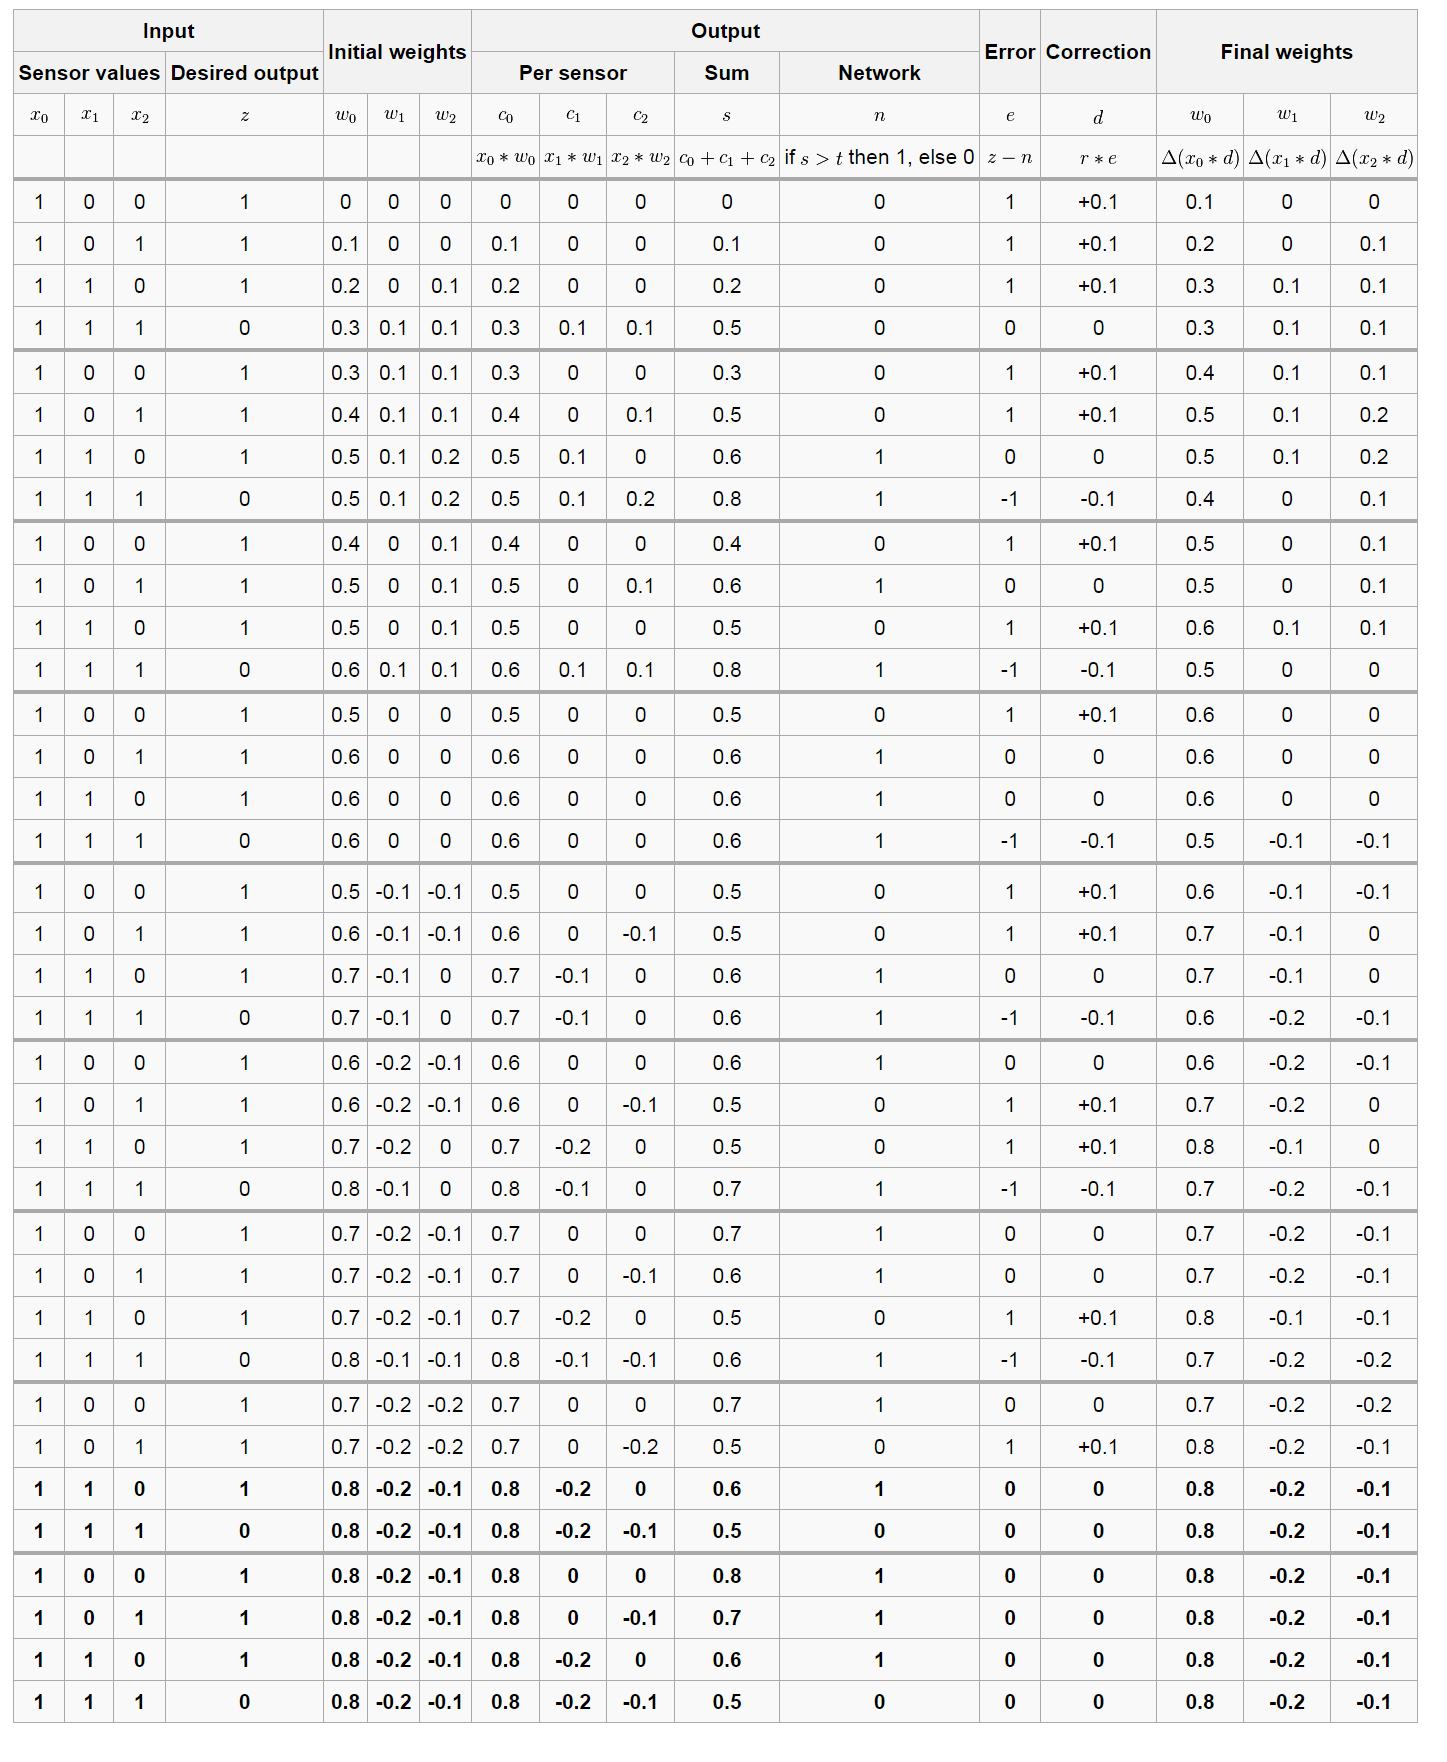
\includegraphics[scale=.5]{./img/example_weight_updates_perceptron_network.png}
\end{figure}

\section{Example : $aja/example/ann/perceptron\_network.cpp$}


In our C++ implementation of this network, we have the following classes: we have separate classes for input neurons and output neurons. The \textbf{input\_neuron} class is for the input neurons. This class has weight and activation as data members. The \textbf{output\_neuron} class is similar and is for the output neuron. It is declared as a friend class in the \textbf{input\_neuron} class. The output neuron class has also a data member called output. There is a network class, which is a friend class in the \textbf{output\_neuron} class. An instance of the network class is created with four input neurons. These four neurons are all connected with one output neuron.

\subsubsection{input\_neuron class}
The member functions of the input\_neuron class are: 
\begin{itemize}
\item A default constructor, 
\item A second constructor that takes a real number as an argument, and 
\item A function that calculates the output of the input neuron. \\
\end{itemize}


The constructor taking one argument uses that argument to set the value of the weight on the connection between the input neuron and the output neuron. The functions that determine the neuron activations and the network output are declared public. The activations of the neurons are calculated with functions defined in the neuron classes. A threshold value is used by a member function of the output neuron to determine if the neuron’s activation is
large enough for it to fire, giving an output of 1.

\subsubsection{Implementation of Functions}


The network is designed to have four neurons in the input layer. Each of them is an object of class input\_neuron, and these are member classes in the class network. There is one explicitly defined output neuron of the class out\_neuron. The network constructor also invokes the neuron constructor for each input layer neuron in the network by providing it with the initial weight for its connection to the neuron in the output layer. The constructor for the output neuron is also invoked by the network constructor, at the same time initializing the output and activation data members of the output neuron each to zero. To make sure there is access to needed information and functions, the output neuron is declared a friend class in the class input\_neuron. The network is declared as a friend class in the class out\_neuron.

\subsubsection{Input/Output}
There are two data files used in this program. One is for setting up the weights, and the other for setting up the input vectors. On the command line, you enter the program name followed by the weight file name and the input file name. 
You can find a file called weight.dat, which contains the following data: \\
2.0 3.0 3.0 2.0 \\
3.0 0.0 6.0 2.0 \\
These are two weight vectors. \\
You can find a file called input.dat with the two data vectors below: \\
1.95 0.27 0.69 1.25 \\
0.30 1.05 0.75 0.19 \\

\subsection{Execution}
\begin{lstlisting}[caption={perceptron\_netwotk.cpp output}] %language=C++, 
example/ann/perceptron_network example/ann/weight.dat example/ann/input.dat

This program is for a perceptron network with  
input layer of 4 neurons, each connected to the 
output neuron.

This example takes Real number as Input Signals
Please enter the number of weights/vectors : 2
This is vector # 1
Please enter a threshold value for 
output neuron, eg 7.0 : 7

Input neuron 1 value is : 1.95 weight is : 2  
and its activation is : 3.9
Input neuron 2 value is : 0.27 weight is : 3  
and its activation is : 0.81
Input neuron 3 value is : 0.69 weight is : 3  
and its activation is : 2.07
Input neuron 4 value is : 1.25 weight is : 2  
and its activation is : 2.5

Output neuron activation is : 9.28

The output neuron activation exceeds the-
threshold value of 7
Output value is 1

This is vector # 2
Please enter a threshold value for 
output neuron, eg 7.0 : 7

Input neuron 1 value is : 0.3 weight is : 3  
and its activation is : 0.9
Input neuron 2 value is : 1.05 weight is : 0  
and its activation is : 0
Input neuron 3 value is : 0.75 weight is : 6  
and its activation is : 4.5
Input neuron 4 value is : 0.19 weight is : 2  
and its activation is : 0.38

Output neuron activation is : 5.78

The output neuron activation is smaller than the- 
threshold value of 7
Output value is 0
\end{lstlisting}


\chapter{XOR Function}
The ability of a Perceptron in evaluating functions was brought into question
when Minsky and Papert proved that a simple function like XOR (the logical
function exclusive or) could not be correctly evaluated by a Perceptron. The
XOR logical function, f(A,B), is as follows: \\

\begin{table} 
\caption{XOR Table}
\label{tab:xor_table}
\begin{tabular}{|l|l|c|}
\hline
A & B & $f(A,b) = XOR(A,B)$ \\
\hline
0 & 0 & 0 \\ 
\hline
0 & 1 & 1 \\ 
\hline
1 & 0 & 1 \\ 
\hline
1 & 1 & 0 \\ 
\hline
\end{tabular}
\end{table}

Minsky and Papert showed that it is impossible to come up with the proper set of weights for the neurons in the single layer of a simple Perceptron to evaluate the XOR function. The reason for this is that such a Perceptron, one with a single layer of neurons, requires the function to be evaluated, to be linearly separable by means of the function values. The concept of \textbf{linear separability} is explained next. But let us show you first why the simple perceptron fails to compute this function.

Since there are two arguments for the XOR function, there would be two
neurons in the input layer, and since the function’s value is one number, there would be one output neuron. Therefore, you need two weights w 1 and w 2 ,and a threshold value  ̧. Let us now look at the conditions to be satisfied by the w’s and the  ̧ so that the outputs corresponding to given inputs would be as for the XOR function.First the output should be 0 if inputs are 0 and 0. The activation works out as 0. To get an output of 0, you need 0 <  ̧. This is your first condition. \ref{tab:conditions_on_weights} shows this and two other conditions you need, and why.

\begin{table} 
\caption{Conditions on Weights}
\label{tab:conditions_on_weights}
\begin{tabular}{|l|l|c|c|}
\hline
Input & Activation & Output & Needed Condition  \\
\hline
0, 0  & 0          & 0      & 0 <               \\ 
\hline
0, 1  & $w_1$      & 1      & $w_1$ >           \\ 
\hline
1, 0  & $w_2$      & 1      & $w_2$ <            \\ 
\hline
1, 1  & $w_1 + w_2$ & 0      & $w_1 + w_2$ <       \\ 
\hline
\end{tabular}
\end{table}

From the first three conditions, you can deduce that the sum of the two weights has to be greater than  ̧, which has to be positive itself. Line 4 is inconsistent with lines 1, 2, and 3, since line 4 requires the sum of the two weights to be less than, This affirms the contention that it is not possible to compute the XOR function with a simple perceptron.

Geometrically, the reason for this failure is that the inputs (0, 1) and (1, 0) with which you want output 1, are situated diagonally opposite each other, when plotted as points in the plane, as shown below in a diagram of the output (1=T,0=F): \\

\begin{tabular}{|c|c|}
\hline
F & T \\ \hline
T & F \\ \hline
\end{tabular}

You can’t separate the T’s and the F’s with a straight line. This means that you cannot draw a line in the plane in such a way that neither (1, 1) ->F nor (0,0)->F is on the same side of the line as (0, 1) ->T and (1, 0)-> T.

\section{Linear Separability}
What linearly separable means is, that a type of a linear barrier or a
separator \textbf{a line in the plane}, or \textbf{a plane in the three-dimensional space}, or \textbf{a hyperplane in higher dimensions} should exist, so that the set of inputs that give rise to one value for the function all lie on one side of this barrier, while on the other side lie the inputs that do not yield that value for the function. A hyperplane is a surface in a higher dimension, but with a linear equation defining it much the same way a line in the plane and a plane in the three-dimensional space are defined.

To make the concept a little bit clearer, consider a problem that is similar but, let us emphasize, not the same as the XOR problem.

\newcommand{\Depth}{4}
\newcommand{\Height}{4}
\newcommand{\Width}{4}
\begin{figure}
\centering
\caption{Separating plane}
\label{fig:separating_plane}
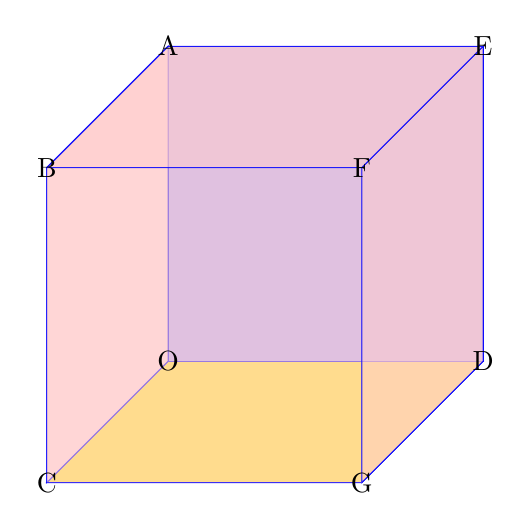
\begin{tikzpicture}
\coordinate (O) at (0,0,0);
\coordinate (A) at (0,\Width,0);
\coordinate (B) at (0,\Width,\Height);
\coordinate (C) at (0,0,\Height);
\coordinate (D) at (\Depth,0,0);
\coordinate (E) at (\Depth,\Width,0);
\coordinate (F) at (\Depth,\Width,\Height);
\coordinate (G) at (\Depth,0,\Height);

\coordinate (1) at (\Depth/2, 0, 0);
\coordinate (2) at (\Depth/2, 0, \Height);
\coordinate (3) at (\Depth/2, \Width, 0);
\coordinate (4) at (\Depth/2, \Width, \Height);

\draw[blue,fill=yellow!80] (O) -- (C) -- (G) -- (D) -- cycle;% Bottom Face
\draw[blue,fill=blue!30] (O) -- (A) -- (E) -- (D) -- cycle;% Back Face
\draw[blue,fill=red!10] (O) -- (A) -- (B) -- (C) -- cycle;% Left Face
\draw[blue,fill=red!20,opacity=0.8] (D) -- (E) -- (F) -- (G) -- cycle;% Right Face
\draw[blue,fill=red!20,opacity=0.6] (C) -- (B) -- (F) -- (G) -- cycle;% Front Face
\draw[blue,fill=red!20,opacity=0.8] (A) -- (B) -- (F) -- (E) -- cycle;% Top Face
%\draw[green,fill=red!20,opacity=0.8] (1) -- (2) -- (3) -- (4) % ToDo: Centre line
% Following is for debugging purposes so you can see where the points are
% These are last so that they show up on top
\foreach \xy in {O, A, B, C, D, E, F, G}{
    \node at (\xy) {\xy};
}
\end{tikzpicture}
\end{figure}

Imagine a cube of 1-unit length for each of its edges and lying in the positive octant in a xyz-rectangular coordinate system with one corner at the origin.
The other corners or vertices are at points with coordinates (0, 0, 1), (0, 1, 0),(0, 1, 1), (1, 0, 0), (1, 0, 1), (1, 1, 0), and (1, 1, 1). Call the origin O, and the seven points listed as C, A, B, D, G, E, and F, respectively. Then any two faces
opposite to each other are linearly separable because you can define theseparating plane as the plane halfway between these two faces and also parallel to these two faces.
For example, consider the faces defined by the set of points O, A, B, and C and
by the set of points D, E, F, and G. They are parallel and 1 unit apart, as you
can see in Figure 5.1. The separating plane for these two faces can be seen to
be one of many possible planes—any plane in between them and parallel to
them. One example, for simplicity, is the plane that passes through the points
(1/2, 0, 0), (1/2, 0, 1), (1/2, 1, 0), and (1/2, 1, 1). Of course, you need only
specify three of those four points because a plane is uniquely determined by
three points that are not all on the same line. So if the first set of points
corresponds to a value of say, +1 for the function, and the second set to a value
of –1, then a single-layer Perceptron can determine, through some training
algorithm, the correct weights for the connections, even if you start with the
weights being initially all 0

Consider the set of points O, A, F, and G. This set of points cannot be linearly
separated from the other vertices of the cube. In this case, it would be
impossible for the single-layer Perceptron to determine the proper weights for
the neurons in evaluating the type of function we have been discussing.
\chapter{References}
Without following links Ctrl + c and Ctrl + v would have not happened!

http://en.wikipedia.org/wiki/Perceptron

